\chapter{Expectation-maximization algorithms}

The generic framework for expectation-maximization (EM) algorithms introduced
by \cite{bucstuvog15} applies to several kinds of probability models, e.~g.,
language models, translation models, and parsing models.
This chapter will introduce terminology and notation from \cite{bucstuvog15} as
far as is necessary to apply this framework to the Hidden Markov model in the
subsequent chapters.

\section{Preliminaries}

The set $\brc{0,1,2,\ldots}$ of non-negative integers and the set of
non-negative reals shall be denoted by $\zn$ and $\zr_{\geq0}$, respectively.
We assume that
\begin{align*}
 0^0 &:= 1, &
 \log 0 &:= -\infty, &
 0 \cdot (-\infty) &= \log 0^0 = 0.
\end{align*}

\begin{definition}
 Given a countable set $X$, a mapping $c\colon X \to \zr_{\geq0}$ is called a
 \emph{$X$-corpus}. Its \emph{size} and \emph{support} are defined as
 \begin{align*}
  \abs c &:= \sum_{x\in X} c(x) &
  \text{and} &&
  \operatorname{supp}(c) &:= \brc{x\in X\colon c(x)\neq0},
 \end{align*}
 respectively. The corpus $c$ is called \emph{empty} if $\abs c = 0$, \emph{finite} if
 $\abs c<\infty$, and \emph{probability distribution of $X$} if $\abs c = 1$.
 The set of all probability distributions of $X$ is denoted by $\um(X)$.
\end{definition}

When used as input for a language model's training algorithm, $X$ is the set of
all sentences consisting of words from the language in question, and $c(x)$
describes how often a sentence $x\in X$ occurs in the corpus $c$.
Probability distributions can be derived from corpora as follows.

\begin{definition}
 Given a non-empty and finite $X$-corpus $c$, the \emph{empirical probability
 distribution} $\tilde c$ is defined as
 \[
  \tilde c(x) = \frac{c(x)}{\abs c}.\qedhere
 \]
\end{definition}

This expression is not well-defined for $\abs c = 0$ or $\abs c = \infty$,
hence the requirement for $c$ to be non-empty and finite.

\begin{definition}
 Given an $X$-corpus $c$ and $p\in\um(X)$, the \emph{likelihood of $c$ under
 $p$} is
 % TODO: Darren says it's confusing to have two definitions for what p(...) means.
 % Maybe use a notation like p[c] for the likelihood? (As a counterpoint,
 % consistency with bucstuvog15 is a huge bonus.)
 \[
  p(c) := \prod_{x\in X} p(x)^{c(x)}. \qedhere
 \]
\end{definition}

The likelihood describes the probability of observing the sentences from the
corpus $c$ when sentences occur with the probability distribution described by
$p$. A training algorithm will take $c$ as an input, and seek to find an
admissible $p$ such that $p(c)$ is maximized. If any $p$ is admissible, then
for non-empty and finite $c$, the optimal choice is $p = \tilde c$ because of
the following lemma.

\begin{lemma}\label{lemma:empirical1}
 Let $c$ be a non-empty and finite $X$-corpus. Then $\tilde c(c) \geq p(c)$ for
 every $p\in\um(X)$.
\end{lemma}

\begin{proof}
 It suffices to show that $\log\tilde c(c) \geq \log p(c)$, since $\log$ is
 monotone. Using Gibbs' inequality,
 \begin{align*}
  \log \tilde c(c)
  &= \sum_{x\in X} c(x) \cdot \log \tilde c(x)
  = \abs c \cdot \sum_{x\in X} \tilde c(x) \cdot \log \tilde c(x) \\
  &\geq \abs c \cdot \sum_{x\in X} \tilde c(x) \cdot \log p(x)
  = \sum_{x\in X} c(x) \cdot \log p(x)
  = p(c)
  \qedhere
 \end{align*}
\end{proof}

However, using $p = \tilde c$ directly is not useful because this probability
distribution is grossly overfitted: It will assign zero probability to any
sentence not in the observed corpus. A useful language model thus limits the
set of admissible $p$ by describing the probability distribution in terms of
\emph{model parameters} $\omega\in\Omega$.

\begin{definition}
 Given a set $\Omega$, an \emph{$\Omega$-probability model for $X$} is a
 mapping $p\colon\Omega\to\um(X)$.
\end{definition}

Instead of $p(\omega)$, we write $p_\omega$. Training shall then find
$\omega\in\Omega$ such that $p_\omega(c)$ is maximized.

\begin{definition}
 Let $f\colon A\to B$ be a mapping from sets $A$ to $B$. The \emph{argmax} of $f$ is the set
 \[
  \argmax_{a\in A} f(a) := \brc{a\in A|\forall a'\in A: f(a) \geq f(a')}.\qedhere
 \]
\end{definition}

\begin{definition}
 Given an $\Omega$-probability model $p$ for $X$, the
 \emph{maximum likelihood estimator} for $p$ is the mapping
 \[
  \mle_p\colon \zr_{\geq0}^X \to \up(\Omega),
  \quad
  c \mapsto \argmax_{\omega\in\Omega} p_\omega(c).\qedhere
 \]
\end{definition}

$\mle_p(c)$ is the set of all $\omega$ with maximal likelihood, but training
only needs to find a single $\hat\omega \in \mle_p(c)$. Computing $\mle_p(c)$
by brute force is typically not tractable because the set $\Omega$ is infinite
(usually countably infinite). However, there is one easily solvable special
case.

\begin{lemma}\label{lemma:empirical2}
 Let $c$ be a finite $X$-corpus, and $p$ a $\Omega$-probability model for $X$.
 If there exists $\hat\omega\in\Omega$ such that $p_{\hat\omega} = \tilde c$,
 then $\hat\omega\in\mle_p(c)$.
\end{lemma}

\begin{proof}
 If $c$ is empty, then $p_\omega(c) = 1$ for every $\omega\in\Omega$, and thus
 $\mle_p(c) = \Omega \ni \hat\omega$. Otherwise, by
 Lemma~\ref{lemma:empirical1}, $p_{\hat\omega}(c) = \tilde c(c) \geq
 p_\omega(c)$ for every $\omega\in\Omega$, and thus $\hat\omega \in \mle_p(c)$.
\end{proof}

\section{Algorithmic skeleton}

\begin{algorithm}[t]
 \caption{Algorithmic skeleton for EM of language models according to \cite{bucstuvog15}}
 \label{alg:skeleton}
 \begin{algorithmic}[1]
  \algorithmheader[Input:] $X$-corpus $c$
  \algorithmheader         $\Omega$-probability model $p$ for $Y\times X$
  \algorithmheader         some initial parameter $\omega_0 \in \Omega_0$ where $\Omega_0 := \brc{\omega\in\Omega: p_\omega(c) \neq 0}$
  \algorithmheader[Implicit:] step mapping $\psi:\Omega_0\to\up(\Omega)$
  \algorithmheader            \hspace{1em} such that $\omega'\in\psi(\omega)$ implies $p_\omega(c) \leq p_{\omega'}(c)$ (\emph{nondecreasing})
  \algorithmheader[Output:] sequence $\omega_1,\omega_2,\ldots\in\Omega_0$
  \algorithmheader            \hspace{1em} such that $p_{\omega_0}(c), p_{\omega_1}(c), p_{\omega_2}(c),\ldots$ nondecreasing

  \STATE $i\leftarrow 0$
  \WHILE{not converged}
   \STATE $\omega_{i+1} \leftarrow \text{select a member of $\psi(\omega_i)$}$
   \STATE output $\omega_{i+1}$
   \STATE $i\leftarrow i+1$
  \ENDWHILE
 \end{algorithmic}
\end{algorithm}

The major complication that occurs when trying to train a language
model is that not all required data is present in the corpus. For example, a
probabilistic context-free grammar is described by the probability distribution
over derivation rules. \cite{laryou90} When the training data consists of full
parse trees (\emph{supervised training}), the optimal probability distribution
can be found by simply counting how many times each rule is used across all
these parse trees, and then computing the empirical probability distribution
for this corpus. Most of the times, however, the training data will consist
only of sentences (\emph{unsupervised training}). The information about how to
parse the sentences is hidden.

The same problem arises with the Hidden Markov model: When training data is not
already annotated with state information, the information about which states
correspond to which words from the training data remains hidden. Expectation
maximization algorithms can be used when parts of the training data are hidden
in such a way. For the remainder, let\label{02-basic-requirements}
\begin{itemize}\setlength\itemsep{-0.3em}
 \item $X$ and $Y$ be countable sets,
 \item $\Omega$ be a set,
 \item $c$ be a finite $X$-corpus and
 \item $p$ be a $\Omega$-probability model for $Y\times X$.
\end{itemize}

The corpus $c$ represents the set of training data. Each $x\in\operatorname{supp}(c)$ is
an \emph{observation}. To judge its probability under any $p_\omega$, additional
\emph{hidden information} $y\in Y$ is required. For notational convenience, we define
\begin{align*}
 p_\omega(c) &:= \prod_{x\in X} p_\omega(x)^{c(x)}, &
 \text{where } p_\omega(x) &:= \sum_{y\in Y} p_\omega(y,x).
\end{align*}

That is, even though $p_\omega$ is a probability distribution over $Y\times X$,
we allow to take the likelihood of the $X$-corpus $c$ under $p$ by aggregating
the probabilities for all hidden information $y$ that lead to a certain
observation $x$ according to the law of total probability.

The basic pattern for expectation maximization is outlined in
Algorithm~\ref{alg:skeleton}. The algorithm starts with an initial $\omega_0$
such that $p_{\omega_0}(c) \neq 0$. It then iteratively employs a step mapping
to choose the next $\omega_i$ with a higher (or at least equal) likelihood than
the one that came before.

\begin{definition}
 Let $\Omega_0 := \brc{\omega\in\Omega: p_\omega(c) \neq 0}$. A \emph{step
 mapping} is a mapping $\psi\colon\Omega_0\to\up(\Omega)$ which is nondecreasing in
 the following manner:
 \[
  \forall \omega\in\Omega_0: \forall \omega'\in\psi(\omega): p_\omega(c) \leq p_{\omega'}(c). \qedhere
 \]
\end{definition}

The step mappings that we will consider will typically consist of two steps:
\begin{enumerate}
 \item \emph{Expectation:} The training data $c$ is converted into a
  \emph{complete-data corpus}. Using $\omega_i$ from the previous
  iteration, the complete-data corpus estimates how hidden information
  contributes to the observations in the original corpus.
 \item \emph{Maximization:} A suitable maximum-likelihood estimator is applied
  to the complete-data corpus to choose $\omega_{i+1}$.
\end{enumerate}

%TODO: this section may use some citations because it makes claims
This back and forth of using the current $\omega$ to enrich the training data
and using the enriched data to find a better $\omega$ will converge towards a
local maximum or saddle point of likelihood. The iteration is usually
aborted after the desired running time has been exceeded, or after the changes
of $p_{\omega_i}(c)$ per iteration have become smaller than some threshold.

\cite{bucstuvog15} identify three types of step mappings that build on each
other, each one more specific than the one before it. Since the training of
Hidden Markov models will be identified as an instance of the most specific
step mapping, the inside-outside step mapping, the remainder of this chapter
will introduce all three in order.

\section{Corpus-based step mapping}

The most general type of complete-data corpus can be obtained by distributing
$c(x)$ among the hidden information $y$ according to the probability
distribution $p_\omega$:
\[
 c\!\dangle{\omega,p}(y,x) := \begin{cases}
  c(x) \cdot \frac{p_\omega(y,x)}{p_\omega(x)} & \text{if } p_\omega(x) \neq 0, \\
  0 & \text{if } p_\omega(x) = 0.
 \end{cases}
\]
Recall that $p_\omega(x) = \sum_y p_\omega(y,x)$. Therefore,
$\abs{c\!\dangle{\omega,p}} = \abs c$. This corpus now has the correct
structure for plugging it into $\mle_p$, yielding the \emph{corpus-based step
mapping}\footnote{The proof that this step mapping is nondecreasing can be
found in \cite[pp.~10]{bucstuvog15}.}
\[
 \stepmap p_\mathrm{cb}\colon \Omega_0\to\up(\Omega),
 \quad
 \omega \mapsto \mle_p\mbig\kla{c\!\dangle{\omega,p}} = \argmax_{\omega'} p_{\omega'}\mbig\kla{c\!\dangle{\omega,p}}.
\]

For very simple language models, the $\argmax$ can be solved at this point
already. To apply Lemma~\ref{lemma:empirical2}, $\hat\omega$ needs to be found
such that $p_{\hat\omega} = \widetilde{c\!\dangle{\omega,p}}$. This operation
is typically hard, which is why a more specific step mapping is helpful.

\section{Simple counting step mapping}

The next such step mapping requires the language model to be described by a
\emph{counting information}. Before defining this term, some additional
notation needs to be introduced.

\begin{definition}\label{def:02-cpd}
 Let $A$ and $B$ be sets. A mapping $p\colon B \to \um(A)$ is called
 \emph{conditional probability distribution of $A$ given $B$}. The set of all
 such mappings is denoted by $\um(A|B)$.
\end{definition}

To simplify notation, we define $p(a|b) := \mbig\kla{p(b)}(a)$.

\begin{definition}\label{def:02-cpd-restr}
 Let $C\subseteq A\times B$ be a set. Then
 \[
  \um_C(A|B) := \mbig\brc{p\in\um(A|B)\!\dmiddle|\! \forall (a,b)\in A\times B\colon (a,b)\notin C \Rightarrow p(a|b) = 0}
 \]
is the \emph{set of all conditional probability distributions of $A$ given $B$
 constrained to $C$}.
\end{definition}

\begin{definition}
 Given a set $\Omega$, a \emph{conditional $\Omega$-probability model for $A$
 and $B$ (constrained to $C$)} is a mapping $q\colon\Omega\to\um(A|B)$ (or
 $q\colon\Omega\to\um_C(A|B)$).
\end{definition}

When talking about counting informations (and inside-outside informations in
the next section), we assume the previously established requirements for $X$,
$Y$, $\Omega$, $c$ and $p$ (see page~\pageref{02-basic-requirements}).
Furthermore, we require that $X$ and $Y$ both contain a special symbol $\bot$
such that $c(\bot) = 0$. $\bot$ can easily be
added to any previously defined $X$ and $Y$ without affecting the requirement
for countability. The notation $U_{\not\bot} := U\setminus\brc\bot$ shall be
defined for any set $U$.

\begin{definition}
 Let $A$, $B$ and $C$ be sets such that $C\subseteq A\times B$. A
 \emph{counting information} is a triple $\varkappa = (q,\lambda,\pi)$ such
 that
 \begin{align*}
  q &\colon \Omega\to\um_C(A|B), &
  \lambda &\colon X_{\not\bot} \times Y_{\not\bot} \to [0,1], &
  \pi &\colon X_{\not\bot} \times Y_{\not\bot} \to \zr_{\geq0}^C.
  \qedhere
 \end{align*}
\end{definition}

The motivation for this definition is to model hidden information $y$ as
consisting of countable events $c\in C$. The mapping $\lambda$ describes
whether (and, possibly, with what probability) a certain $y$ can be the cause
for a certain observation $x$.\footnote{Most instances of $\lambda$ use only
integer images, i.~e.~$\lambda(X_{\not\bot}\times Y_{\not\bot}) = \brc{0,1}$,
thus following this intuitive notion. However, the possibility of using
fractional values for $\lambda(x,y)$ is occasionally useful, e.~g.~to define a
counting information for the IBM Model 1 in \cite[pp.~23]{bucstuvog15}.} For
$\lambda(x,y)>0$, the $C$-corpus $\pi(x,y)$ describes how often each countable
event occurs in this hidden information.

Following the assumption that the countable events $C$ fully encode the hidden
information $Y$, we can use these intuitive notions to describe the original
probability model $p$ in terms of the counting information.

\pagebreak
\begin{definition}
 Given $\varkappa=(q,\lambda,\pi)$, the \emph{induced model}
 $\varkappa^\flat\colon\Omega\to\zr^{Y\times X}$ is given by
 \[
  (\varkappa^\flat)_\omega(y,x) := \begin{cases}
   \lambda(x,y) \cdot q_\omega\mbig\kla{\pi(x,y)} & \text{if } x,y\neq\bot, \\
   1 - \sum_{x',y'\neq\bot} \lambda(x',y') \cdot q_\omega\mbig\kla{\pi(x',y')} & \text{if } x = y = \bot, \\
   0 & \text{otherwise}.
  \end{cases}\qedhere
 \]
\end{definition}

This shows why the introduction of $\bot$ into $X$ and $Y$ was useful. The
definition ensures that $\mnorm\abs{(\varkappa^\flat)_\omega} = 1$. Therefore,
$\varkappa^\flat$ is an $\Omega$-probability model for $Y\times X$ iff
$(\varkappa^\flat)_\omega(\bot,\bot) \geq 0$. We call $\varkappa$ \emph{proper}
in this case.

Since we now have a probability model $p = \varkappa^\flat$ as required by the
corpus-based step mapping, we can lift its complete-data corpus into the domain
of the counting information, obtaining a new complete-data corpus
\[
 c\!\dangle{\omega,\varkappa}\colon C \to \zr_{\geq0}, \quad
 (a,b) \mapsto \sum_{x,y} c\mnorm\dangle{\omega,\varkappa^\flat}(y,x) \cdot \mbig\kla{\pi(x,y)}(a,b).
\]

\begin{definition}
 Given a set $\Omega$ and a conditional $\Omega$-probability model $q$ for $A$
 and $B$, the \emph{conditional maximum likelihood estimator} for $q$ is the mapping
 \[
  \cmle_q\colon \zr_{\geq0}^{A\times B} \to \up(\Omega),
  \quad
  c \mapsto \argmax_\omega q_\omega(c). \qedhere
 \]
\end{definition}

Using this definition, the \emph{simple counting step mapping} is
\[
 \stepmap\varkappa_\mathrm{sc}\colon \Omega_0 \to \up(\Omega), \quad
 \omega \mapsto \cmle_q\mbig\kla{c\mnorm\dangle{\omega,\varkappa}} = \argmax_{\omega'} q_{\omega'}\mbig\kla{c\mnorm\dangle{\omega,\varkappa}}.
\]
\cite[p.~13]{bucstuvog15} show that this step mapping is
equivalent to $\mnorm\stepmap{\varkappa^\flat}_\mathrm{cb}$, and thus also
nondecreasing.
The simple counting step mapping has two advantages over
$\stepmap\cdot_\mathrm{cb}$: First, many language models can be described in
terms of the countable events only, such that $\Omega = C$. In this case,
Lemma~\ref{lemma:empirical2} can be used to solve the $\argmax$ by computing
the empirical probability distribution of $c\!\dangle{\omega,\varkappa}$.

Second, even if this is not possible, the set of countable events $C$ is
usually much smaller than the set of all observations $X$ or hidden information
$Y$, making the evaluation of the $\argmax$ more tractable than for the
corpus-based step mapping. For example, when considering probabilistic
context-free grammars, $X$ (the set of all sentences) and $Y$ (the set of all
parse trees) are both countably infinite, but $C$ (the set of all derivation
rules) is finite.

\section{Regular tree grammars}

The third and most specific type of step mapping applies to language models
whose hidden information can be described as trees, such that the countable
events are labels in these trees' nodes. We therefore need to introduce some
terminology regarding alphabets and trees first.

\begin{definition}
 An \emph{alphabet} is a finite set. Its elements are called \emph{letters}.
\end{definition}

Terminology and notation regarding alphabets will be useful both for the
definition of trees in this chapter and for the discussion of the Hidden Markov
model in the next chapter.\footnote{The terms ``alphabet'', ``letters'' and
``words'' are commonly used in formal language theory to describe a set of base
symbols, its elements and strings of them. However, in natural language
processing, the individual symbols are words rather than letters, and their
strings are sentences rather than words. These terms will consequently be
applied in chapter 3 and beyond.}

\begin{definition}
 Let $\Sigma$ be an alphabet. For any $n\in\zn$, a sequence $\sigma =
 \sigma_1\cdots\sigma_n$ of letters $\sigma_1,\ldots,\sigma_n\in\Sigma$ is
 called a \emph{word} over $\sigma$ with \emph{length} $\abs\sigma = n$. For
 $n=0$, the \emph{empty word} is denoted by $\eps$. Given two words
 $\sigma=\sigma_1\cdots\sigma_n$ and $\tau=\tau_1\cdots\tau_m$, their
 \emph{concatenation} is the word
 \[
  \sigma\tau := \sigma_1\cdots\sigma_n\tau_1\cdots\tau_m,
 \]
 and especially $\sigma\eps := \sigma$ and $\eps\tau := \tau$. The
 concatenation of two sets $S$ and $T$ of words over $\Sigma$ is
 \[
  S\cdot T := \brc{\sigma\tau|\sigma\in S, \tau\in T}.\qedhere
 \]
\end{definition}

In this regard, the alphabet $\Sigma$ can be considered to be a set of words
since letters are isomorphic to one-letter words.

\begin{definition}
 Let $\Sigma$ be an alphabet. The \emph{Kleene star} of $\Sigma$ is the set of
 all words over $\Sigma$, i.~e.,
 \[
  \Sigma^* := \bigcup_{i=0}^\infty \Sigma^i, \quad
  \text{where }\Sigma^i := \begin{cases}
   \brc\eps & \text{if } i = 0, \\
   \Sigma^{i-1}\cdot\Sigma & \text{otherwise}.
  \end{cases}\qedhere
 \]
\end{definition}

We also use $\Sigma^+ := \Sigma^* \setminus\brc{\eps}$ to refer to the set of
\emph{nonempty words} over $\Sigma$.

\begin{definition}
 Let $\Sigma$ be an alphabet and $V$ be a set such that $\Sigma\cap
 V=\emptyset$. The \emph{set $U_\Sigma(V)$ of unranked trees over $\Sigma$
 indexed by $V$} is the smallest set $T$ such that
 \[
  V \subseteq T \quad\text{and}\quad \forall k\in\zn: \forall \sigma\in\Sigma, t_1,\ldots,t_k\in T: \sigma(t_1,\ldots,t_k)\in T.
  \qedhere
 \]
\end{definition}

The notation $\sigma(t_1,\ldots,t_k)$ refers to the tree which has the label
$\sigma$ at its root and the subtrees $t_1,\ldots,t_k$ in that order. For
$k=0$, we write $\sigma$ instead of $\sigma()$. For $V=\emptyset$, we write
$U_\Sigma$ instead of $U_\Sigma(\emptyset)$. Trees from $U_\Sigma(V)$ have
labels from $\Sigma\cup V$ at each node, but labels from $V$ are only permitted
at leaves (see Figure~\ref{fig:02-trees1}). We refer to positions in the tree
using \emph{Gorn notation}.

\begin{figure}[t!]
 \[\begin{matrix}
  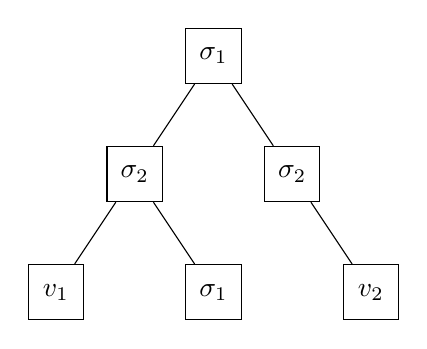
\begin{tikzpicture}[every node/.style={rectangle,draw,minimum size=2em},baseline=(current bounding box.center)]
   \node (n)   at (+0,+0.0) { $\sigma_1$ };
   \node (n1)  at (-1,-1.5) { $\sigma_2$ } edge (n);
   \node (n2)  at (+1,-1.5) { $\sigma_2$ } edge (n);
   \node (n11) at (-2,-3.0) { $v_1$ } edge (n1);
   \node (n12) at (+0,-3.0) { $\sigma_1$ } edge (n1);
   \node (n21) at (+2,-3.0) { $v_2$ } edge (n2);
  \end{tikzpicture}
  &\hspace*{4em}&
  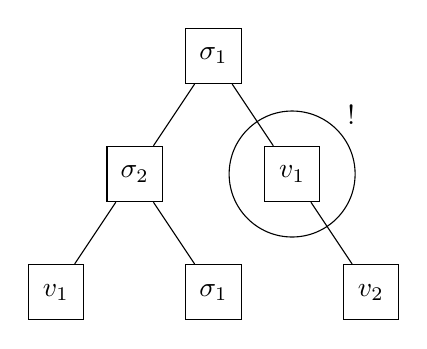
\begin{tikzpicture}[every node/.style={rectangle,draw,minimum size=2em},baseline=(current bounding box.center)]
   \node (n)   at (+0,+0.0) { $\sigma_1$ };
   \node (n1)  at (-1,-1.5) { $\sigma_2$ } edge (n);
   \node (n2)  at (+1,-1.5) { $v_1$ } edge (n);
   \node (n11) at (-2,-3.0) { $v_1$ } edge (n1);
   \node (n12) at (+0,-3.0) { $\sigma_1$ } edge (n1);
   \node (n21) at (+2,-3.0) { $v_2$ } edge (n2);
   \draw (n2) circle (0.8);
   \node[draw=none] at (+1.75,-0.75) {!};
  \end{tikzpicture}
  \\\\
  \sigma_1\mbig\kla{\sigma_2(v_1,\sigma_1), \sigma_2(v_2)} \in U_\Sigma(V) &&
  \sigma_1\mbig\kla{\sigma_2(v_1,\sigma_1), v_1(v_2)} \notin U_\Sigma(V)
 \end{matrix}\]
 \caption{
  Example (left) and counter-example (right) for trees from $U_\Sigma(V)$,
  where $\Sigma = \{\sigma_1,\sigma_2\}$ and $V = \{v_1,v_2\}$.
  \label{fig:02-trees1}
 }
\end{figure}

\begin{definition}
 Given $t\in U_\Sigma(V)$, the set of \emph{positions} in $t$ is defined recursively by
 \[
  \pos(t) := \begin{cases}
   \brc\eps & t = v\in V, \\
   \brc\eps\cup \bigcup_{i=1}^k \brc{i} \cdot \pos(t_i) & t = \sigma(t_1,\ldots,t_k).
  \end{cases}
  \qedhere
 \]
\end{definition}

Positions are words from $\zn^*$. Figure~\ref{fig:02-trees2} illustrates the
set of positions in a tree, and some of the operations on positions as defined
below.

\begin{figure}[t!]
 \vspace*{-1em}\[
  \hspace*{3em}
  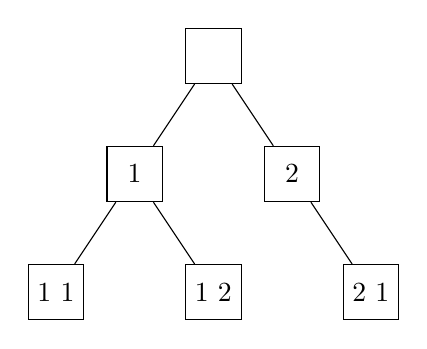
\begin{tikzpicture}[every node/.style={rectangle,draw,minimum size=2em},baseline=(current bounding box.center)]
   \node (n)   at (+0,+0.0) { $\eps$ };
   \node (n1)  at (-1,-1.5) { $1$ } edge (n);
   \node (n2)  at (+1,-1.5) { $2$ } edge (n);
   \node (n11) at (-2,-3.0) { $1\ 1$ } edge (n1);
   \node (n12) at (+0,-3.0) { $1\ 2$ } edge (n1);
   \node (n21) at (+2,-3.0) { $2\ 1$ } edge (n2);
  \end{tikzpicture}
  \hspace*{6em}
  \begin{tikzpicture}[baseline=(current bounding box.center)]
   \begin{scope}[every node/.style={rectangle,draw,fill=white,minimum size=2em}]
    \node (n)   at (+0,+0.0) { $\sigma_1$ };
    \node (n1)  at (-1,-1.5) { $\sigma_2$ } edge (n);
    \node (n2)  at (+1,-1.5) { $\sigma_2$ } edge (n);
    \node (n11) at (-2,-3.0) { $v_1$ } edge (n1);
    \node (n12) at (+0,-3.0) { $\sigma_1$ } edge (n1);
    \node (n21) at (+2,-3.0) {} edge (n2);
   \end{scope}
   \begin{scope}[every node/.style={inner sep=0},every pin/.style={inner sep=0},pin distance=1cm]
    \node[draw=none,pin=60:{$t(2\ 1)$}] at (n21.center) { $v_2$ };
   \end{scope}
   \begin{scope}[on background layer]
    \draw[line join=round,draw=black!10,fill=black!10,line width=1.5cm] (n1.center) -- (n11.center) -- (n12.center) -- cycle;
   \end{scope}
   \node at (-2.4,-1.7) { $t|_1$ };
  \end{tikzpicture}
 \]
 \caption{
  Left: A tree from $U_{\zn^*}$ in which every node is labeled with its
  position within the tree. Right: Illustration of the operations $t(w)$ and
  $t|_w$ for a tree $t$ and positions $w\in\pos(t)$.
  \label{fig:02-trees2}
 }
\end{figure}

\begin{definition}
 Given $t\in U_\Sigma(V)$ and $w\in\pos(t)$, $t(w)$ denotes the \emph{label} in $t$ at position $w$, i.~e.,
 \[
  t(w) := \begin{cases}
   v & t = v\in V \text{ and } w=\eps, \\
   \sigma & t = \sigma(t_1,\ldots,t_k) \text{ and } w = \eps, \\
   t_i(w') & t = \sigma(t_1,\ldots,t_k) \text{ and } w = iw' \text{ where } i\in\zn, w'\in\pos(t_i).
  \end{cases}
 \]
 where $i\in\zn$ and $w'\in\pos(t_i)$. Moreover, $t|_w$ denotes the \emph{subtree} in $t$ at position $w$, i.~e.,
 \[
  t|_w := \begin{cases}
   t & w = \eps, \\
   t_i|_{w'} & t = \sigma(t_1,\ldots,t_k) \text{ and } w = iw',
  \end{cases}
 \]
 and for any $t'\in U_\Sigma(V)$, $t[t']_w$ denotes the tree that results from replacing $t|_w$ by $t'$, i.~e.,
 \[
  t[t']_w := \begin{cases}
   t' & w = \eps, \\
   \sigma(t_1,\ldots,t_{i-1},t_i[t']_{w'},t_{i+1},t_k) & t = \sigma(t_1,\ldots,t_k) \text{ and } w = iw'.
  \end{cases}
 \]
 %TODO: Gibt es hierfür eine Standard-Notation? Wird nur noch einmal unten verwendet bei der Einführung von T_R.
 Finally, $\osucc(t)$ denotes the set of \emph{successors} of $t$, i.~e.,
 \[
  \osucc(t) := \begin{cases}
   \emptyset & t = v\in V, \\
   \brc{t_1,\ldots,t_k} & t = \sigma(t_1,\ldots,t_k).
  \end{cases}
  \qedhere
 \]
\end{definition}

\begin{definition}
 Let $\Sigma$ be an alphabet and $\square\notin\Sigma$ be some symbol. A
 \emph{1-context over $\Sigma$} is a tree $t\in U_\Sigma(\brc\square)$ such
 that $\square$ appears at exactly one position in $t$. The set of all such
 1-contexts is denoted by $C_\Sigma$.
\end{definition}

\pagebreak

1-contexts are used to describe trees that are not fully known yet: The
symbol $\square$ is a placeholder for a missing subtree. Given a 1-context
$t\in C_\Sigma$ and a tree $t'\in U_\Sigma(V)$, we abbreviate $t[t'] :=
t[t']_w$ such that $t(w) = \square$. In other words, $t[t']$ is the tree that
results from $t$ when the node labeled with $\square$ is replaced by $t'$.

\begin{definition}
 A \emph{ranked alphabet} is a pair $(R,\rk)$ where $R$ is an alphabet and
 $\rk\colon R\to\zn$ is a mapping. $\rk$ is said to assign a \emph{rank} or
 \emph{arity} to each symbol in $R$.
\end{definition}

A ranked alphabet is usually denoted only by $R$. The existence of a suitable
$\rk$ is implied.

\begin{definition}
 Let $R$ be a ranked alphabet and $V$ be a set. The \emph{set $T_R(V)$ of
 ranked trees over $R$ indexed by $V$} is defined by
 \[
  T_R(V) := \mbig\brc{t \in U_R(V) \dmiddle| \forall w\in\pos(t): t(w)\in R\Rightarrow \rk\mbig\kla{t(w)} = \mbig\abs{\osucc\mbig\kla{t|_w}}}.
  \qedhere
 \]
\end{definition}

In other words, the number of children of each node in $t$ with a label from
$R$ must be equal to the rank of that label.

\begin{definition}
 Given an alphabet $\Sigma$, a \emph{regular tree grammar (RTG) over $\Sigma$}
 is a triple $\ug = (Q,q_0,R)$ where $Q$ is a nonempty alphabet (of states),
 $q_0\in Q$ is an initial state, and $R\subset Q^*\times\Sigma\times Q$ is a
 finite ranked alphabet (of rules) such that
 \[
  \forall \rho = \mbig\kla{(q_1,\ldots,q_k),\sigma,q}\in R\colon \rk(\rho) = k.
  \qedhere
 \]
\end{definition}

We will write $\mbig\kla{(q_1,\ldots,q_k),\sigma,q}$ as $q\to\sigma(q_1,\ldots,q_k)$.

\begin{definition}
 Let $\ug=(Q,q_0,R)$ be an RTG. The \emph{family
 $\mbig\kla{D^q(\ug)\!\dmiddle|\!q\in Q}$ of partial abstract syntax trees of
 $\ug$} is the smallest $Q$-indexed family $(D^q|q\in Q)$ such that, for all
 $q\in Q$,
 \[
  q \in D^q \quad\text{and}\quad \forall \rho=\mbig\kla{q\to\sigma(q_1,\ldots,q_k)}\in R,d_1\in D^{q_1},\ldots,d_k\in D^{q_k}: \rho(d_1,\ldots,d_k) \in D^q.
 \]
 An \emph{abstract syntax tree} is a partial abstract syntax tree $d\in
 D^{q_0}(\ug)$ that does not have any nodes labeled with symbols from $Q$.
\end{definition}

An RTG generates a language (i.~e.,~a countable set) of trees. Trees are derived
by starting with a tree containing only the a root node with the label $q_0$,
then successively replacing $Q$-labeled nodes according to the RTG's rule set
until no more $Q$-labeled nodes are left. The resulting tree is in $U_\Sigma$
and its abstract syntax tree is in $T_R$. Partial abstract syntax trees are in $T_R(Q)$.
For example, consider the RTG $\ug = \mbig\kla{\brc{q_0,q_1},q_0,R}$ where
$\Sigma=\brc{a,b,c}$ and
\[
 R = \brc{ q_0 \to a(q_0,q_1), \quad q_0 \to b, \quad q_1 \to c }.
\]
The tree $a(b,c)$ is derived like this: (Each row shows the partial tree from
$U_\Sigma(Q)$ on the left and the partial abstract syntax tree from $T_R(Q)$ on
the right.)
\[\begin{matrix}
 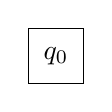
\begin{tikzpicture}[every node/.style={rectangle,draw,minimum size=2em},baseline=(current bounding box.center)]
  \node (n) at (0,0) { $q_0$ };
 \end{tikzpicture}
 &&
 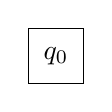
\begin{tikzpicture}[every node/.style={rectangle,draw,minimum size=2em},baseline=(current bounding box.center)]
  \node (n) at (0,0) { $q_0$ };
 \end{tikzpicture}
 \\\\[-1em]
 \downarrow & \text{apply } q_0\to a(q_0,q_1) & \downarrow \\[0.5em]
 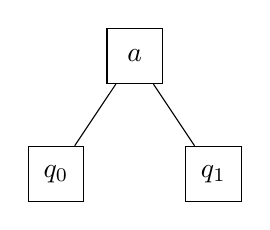
\begin{tikzpicture}[every node/.style={rectangle,draw,minimum size=2em},baseline=(current bounding box.center)]
  \node (n) at (0,0) { $a$ };
  \node (n1) at (-1,-1.5) { $q_0$ } edge (n);
  \node (n2) at (+1,-1.5) { $q_1$ } edge (n);
 \end{tikzpicture}
 &\hspace*{4em}&
 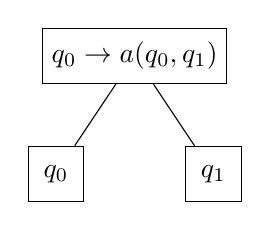
\begin{tikzpicture}[every node/.style={rectangle,draw,minimum size=2em},baseline=(current bounding box.center)]
  \node (n) at (0,0) { $q_0 \to a(q_0,q_1)$ };
  \node (n1) at (-1,-1.5) { $q_0$ } edge (n);
  \node (n2) at (+1,-1.5) { $q_1$ } edge (n);
 \end{tikzpicture}
 \\\\[-1em]
 \downarrow & \text{apply } q_0\to b & \downarrow \\[0.5em]
 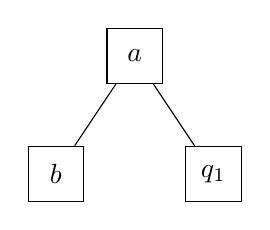
\begin{tikzpicture}[every node/.style={rectangle,draw,minimum size=2em},baseline=(current bounding box.center)]
  \node (n) at (0,0) { $a$ };
  \node (n1) at (-1,-1.5) { $b$ } edge (n);
  \node (n2) at (+1,-1.5) { $q_1$ } edge (n);
 \end{tikzpicture}
 &\hspace*{4em}&
 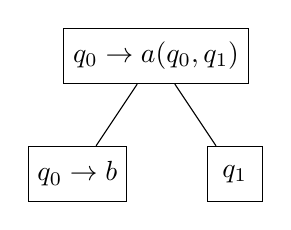
\begin{tikzpicture}[every node/.style={rectangle,draw,minimum size=2em},baseline=(current bounding box.center)]
  \node (n) at (0,0) { $q_0 \to a(q_0,q_1)$ };
  \node (n1) at (-1,-1.5) { $q_0\to b$ } edge (n);
  \node (n2) at (+1,-1.5) { $q_1$ } edge (n);
 \end{tikzpicture}
 \\\\[-1em]
 \downarrow & \text{apply } q_1\to c & \downarrow \\[0.5em]
 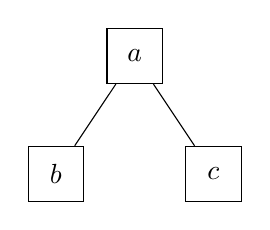
\begin{tikzpicture}[every node/.style={rectangle,draw,minimum size=2em},baseline=(current bounding box.center)]
  \node (n) at (0,0) { $a$ };
  \node (n1) at (-1,-1.5) { $b$ } edge (n);
  \node (n2) at (+1,-1.5) { $c$ } edge (n);
 \end{tikzpicture}
 &\hspace*{4em}&
 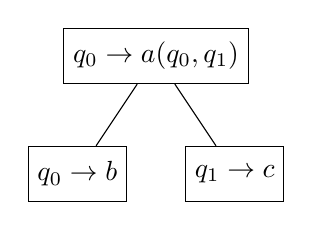
\begin{tikzpicture}[every node/.style={rectangle,draw,minimum size=2em},baseline=(current bounding box.center)]
  \node (n) at (0,0) { $q_0 \to a(q_0,q_1)$ };
  \node (n1) at (-1,-1.5) { $q_0\to b$ } edge (n);
  \node (n2) at (+1,-1.5) { $q_1\to c$ } edge (n);
 \end{tikzpicture}
\end{matrix}\]

From the (partial) abstract syntax tree on the right, the tree on the left can be derived easily
by substituting the labels $q = \sigma(q_1,\ldots,q_k)\in R$ by the contained
symbols $\sigma\in\Sigma$, without changing labels from $Q$. We shall call this
projection $\pi_\Sigma: T_R(Q)\to U_\Sigma(Q)$.

\begin{definition}
 Let $\ug$ be an RTG over $\Sigma$. The \emph{language of $\ug$} is the set
 \[
  \lang\ug := \brc{t\in U_\Sigma | \exists d\in D^{q_0}(\ug)\colon t=\pi_\Sigma(d)}.
 \]
 A language $L\subseteq U_\Sigma$ is \emph{regular} if there exists an RTG
 $\ug$ over $\Sigma$ such that $\lang\ug = L$.
\end{definition}

\pagebreak

A useful property of RTGs is \emph{determinism}: An RTG $\ug$ over $\Sigma$ is
called \emph{deterministic} if, for any $(q_1,\ldots,q_k)\in Q^*$ and
$\sigma\in\Sigma$, there is at most one $q\in Q$ such that $\mbig\kla{q \to
\sigma(q_1,\ldots,q_k)} \in R$. A language is called deterministic if it is
described by a deterministic RTG.

\label{lemma:02-deterministic-is-unambiguous}
From determinism results unambiguity: An RTG $\ug$ over $\Sigma$ is called
\emph{unambiguous} if, for every tree $t\in\lang\ug$, there exists exactly one
abstract syntax tree $d\in D^{q_0}(\ug)$ such that $\pi_\Sigma(d) = t$. To see why, have
a look at the fully derived tree $t = a(b,c)$ above. Since $\ug$ in this
example is deterministic, the abstract syntax tree can be recovered from $t$ by
traversing the nodes from the bottom up and assigning the rules that are used
at that position. At each position, we know the symbol $\sigma$ at this
position in the tree and the states $q_1,\ldots,q_k$ from the left sides of the
rules used for the child nodes. Therefore, the state $q$ (and therefore the
rule $\rho$) for this position can be chosen deterministically.

\begin{definition}
 A \emph{probabilistic regular tree grammar (PRTG) over $\Sigma$} is a pair
 $(\ug,p)$ of an RTG $\ug=(Q,q_0,R)$ over $\Sigma$ and a mapping
 $p:Q\to\zr_{\geq0}^{Q^*\times\Sigma}$ that is constrained to $R$ in the
 following way:
 \[
  \forall q\in Q, u\in Q^*\times\Sigma: \mbig\kla{p(q)}(u) \neq 0 \Rightarrow (u,q) \in R.
 \]
 $(\ug,p)$ is called \emph{proper} if $p\in\um_R(Q^*\times\Sigma|Q)$. The
 \emph{meaning} of $(\ug,p)$ is the mapping
 \[
  \mbig\lang{(\ug,p)}\colon U_\Sigma \to \zr_0, \quad
  t \mapsto \sum_{d\in D^{q_0}(\ug): \pi_\Sigma(d)=t} p(d).
 \]
 Herein, $p(d) := p\mbig\kla{\pi(d)}$, where $\pi(d)$ is an $R$-corpus with
 \[
  \mbig\kla{\pi(d)}(p) := \mbig\abs{\mbig\brc{w\in\pos(d): d(w)=p}}.
 \]
 The set of all \emph{unambiguous} PRTG over $\Sigma$ shall be denoted as $\ur(\Sigma)$.
\end{definition}

We usually write a PRTG $(\ug,p)$ as just $\ug$ and imply the existence of $p$.
The meaning function assigns a probability to a tree from $\lang\ug$ by summing
the probability of all derivations resulting in that tree, where the
probability of a derivation is the product of the probability of each rule
occurring in it. This implies that rule applications are statistically
independent from each other.

When describing hidden information in terms of PRTG in the next section, the
notion of \emph{inside and outside weights} will be useful to judge, broadly
speaking, how much a certain state contributes to the derivations of a certain
observation.

\begin{definition}
 Let $\ug = (Q,q_0,R)$ be a PRTG. The \emph{inside weight} of a state $q\in Q$
 is given by
 \[
  \beta(q) := \sum_{d\in D^q(\ug)\cap T_R} p(d).
  \qedhere
 \]
\end{definition}

The sum goes over all complete abstract syntax trees rooted at $q$. The inside weight
describes the collective probability of all derivations starting at $q$. Inside
weights are usually calculated by noting that each $d\in D^q(\ug)\cap T_R$ must
have a rule of the form $q\to\ldots$ at its root. The remaining probabilities
can then be expressed as the inside weights of the states that emerge from this
rule application, giving
\[
 \beta(q) = \sum_{q_1,\ldots,q_k,\sigma} p\mbig\kla{q\to\sigma(q_1,\ldots,q_k)} \cdot \beta(q_1) \cdots \beta(q_k).
\]

The set of all such equations is a non-linear equation system in the variables $\beta(q)$
for $q\in Q$. In some cases, this system can be solved intuitively by starting
with those equations where no $\beta(q_i)$ occurs on the right-hand side, then
substituting the obtained value in the other equations until they are all
solved. This is not possible, however, if states derive other states in a
cyclic way. For example:
\[
 R = \brc{\begin{aligned}
  \rho_1 &= q_0 \to \sigma_1(q_1, q_1), \\
  \rho_2 &= q_1 \to \sigma_2(q_0), \\
  \rho_3 &= q_1 \to \sigma_3
 \end{aligned}} \quad\leadsto\quad
 \begin{aligned}
  \beta(q_0) &= p(\rho_1) \cdot \beta(q_1)^2 \\
  \beta(q_1) &= p(\rho_2) \cdot \beta(q_0) + p(\rho_3)
 \end{aligned}
\]

In the general case, \cite[pp.~6]{bucstuvog15} show that the inside weights
$\beta$ are the least fixpoint of the mapping $F: (\zr_{\geq0}\cup\brc\infty)^Q
\to (\zr_{\geq0}\cup\brc\infty)^Q$, given by
\[
 \mbig\kla{F(u)}(q) := \sum_{q_1,\ldots,q_k,\sigma} p\mbig\kla{q\to\sigma(q_1,\ldots,q_k)} \cdot u(q_1) \cdots u(q_k).
\]
Therefore,
\[
 \beta = \lim_{n\to\infty} F^n(u_0) \quad\text{where}\quad u_0(q) := 0 \;\forall q\in Q
\]
can be approximated by performing as many iterations of $F$ as desired.

\begin{definition}
 Let $\ug = (Q,q_0,R)$ be a PRTG. The \emph{outside weight} of a state $q\in Q$ is given by
 \[
  \alpha(q) := \sum_{d\in D^{q_0}(\ug): \exists d'\in C_R: d = d'[q]} p(d).
  \qedhere
 \]
\end{definition}

The sum goes over all partial abstract syntax trees starting from $q_0$, where
only one unexpanded state is left, and that state is $q$. The outside weight
describes the collective probability of all derivations that use $q$, but
without considering derivations at or below $q$. Similar to what we did with
inside weights, we can expand this definition into
\[
 \alpha(q) = \delta_{q_0}^q + \sum_{q',q_1,\ldots,q_k,\sigma,m:q_m=q} \alpha(q') \cdot p\mbig\kla{q'\to\sigma(q_1,\ldots,q_k)} \cdot \prod_{l\neq m} \beta(q_l).
\]

In this formulation, the sum goes over all rules that derive $q$, that is, $q$
is among the states $q_1,\ldots,q_k$ on the right hand side of the rule, at
index $m$. The outside weight $\alpha(q)$ considers the outside weight
$\alpha(q')$ of the previous state and the inside weight of all states adjacent
to $q$, but not the inside weight of $q$ itself.

Finally, we need to account for $q=q_0$, in which case the trivial tree $d$ containing only a $q_0$-labeled root node must be considered. Since $p(d)=1$ for this tree, it is accounted for in the above formula through the Kronecker symbol
\[
 \delta_{q_0}^q := \begin{cases}
  1 & \text{if } q_0 = q, \\
  0 & \text{otherwise}.
 \end{cases}
\]

Assuming that the inside weights $\beta(q)$ have already been calculated, the
equations for $\alpha(q)$ form a linear equation system that can be solved
efficiently with the standard algorithms for linear equation systems.

\section{Inside-outside step mapping}

We can now resume the task of describing hidden information in terms of trees,
such that the countable events, as introduced by the counting information, are
labels in these trees' nodes. Similar to how a language model can be described
as a counting information for use with the simple counting step mapping, a
language model may also be described as an inside-outside information, for use
with the inside-outside step mapping.

Again, we assume the previous definitions of $X$, $Y$, $c$, $A$, $B$ and $C$
throughout this section.

\begin{definition}\label{02:def-io-info}
 An \emph{inside-outside (IO) information} is a quadruple\footnote{The definitions
 in this chapter have previously diverged from \cite{bucstuvog15} by omitting
 the set $Z$, which is only required for translation models, and otherwise set
 to $Z=\brc\emptyset$ for language models. For IO informations, this leads to
 additional divergence from the definition in \cite{bucstuvog15}, where $\mu$
 is introduced as a quintuple $\mu=(q,\pi_1,\pi_2,K,H)$. Both definitions are
 congruent for language models by letting $\pi_2(y) :=
 \emptyset\in Z$.} $\mu = (q,\pi_1,K,H)$ such that
 \begin{itemize}\setlength\itemsep{-0.3em}
  \item $C\subseteq A\times B$ is a ranked alphabet such that $Y_{\not\bot}\subseteq T_C$ contains ranked trees over $C$,
  \item $q\colon\Omega\to\um_C(A|B)$ as for counting informations,
  \item $\pi_1\colon Y_{\not\bot}\to X_{\not\bot}$ maps hidden information to observations,
  \item $K\in\ur(C)$ is a unambiguous RTG with $\lang K = Y_{\not\bot}$ and
  \item $H\colon X_{\not\bot}\to\ur(C)$ assigns an unambiguous RTG to every observation such that 
   \[
    \forall x\in X_{\not\bot}\colon \lang{H(x)} = \pi_1^{-1}(x).
   \]
 \end{itemize}
 Furthermore, we require that, for every $\omega\in\Omega$, the PRTG $(K,p'_\omega)$ is proper, where
 \[
  p'_\omega\mbig\kla{q\to(a,b)(q_1,\ldots,q_k)} = q_\omega(a|b).
  \qedhere
 \]
\end{definition}

Each hidden information $y$ is a tree from $T_C$, and a conditional probability
$q_\omega(a|b)$ can be assigned to each countable event $c = (a,b)$ that occurs
in the tree. Each hidden information $y$ belongs to exactly one observation
$x$. The set of all hidden informations $Y_{\not\bot}$ is generated by the PRTG
$(K,p_\omega')$, and for each observation $x$, the set of all hidden
informations leading to this observation is generated by the PRTG
$\mbig\kla{H(x),p_\omega'}$.

The description of a language model using an IO information is a special case of
the description via counting informations, since an IO information induces a
counting information.

\begin{definition}
 Let $\mu=(q,\pi_1,K,H)$ be an IO information. The \emph{induced counting
 information} $\mu^\flat = (q,\lambda,\pi)$ is given by
 \begin{align*}
  \lambda(x,y) &:= \begin{cases}
   1 & \text{if } \pi_1(y) = x, \\
   0 & \text{otherwise},
  \end{cases} \\
  \mbig\kla{\pi(x,y)}(a,b) &:= \begin{cases}
   \mbig\abs{\mbig\brc{w\in\pos(y): y(w)=(a,b)}} & \text{if } \pi_1(y) = x, \\
   0 & \text{otherwise}.
  \end{cases}
  \qedhere
 \end{align*}
\end{definition}
The induced counting information $\mu^\flat$ is always proper.
\cite[p.~15]{bucstuvog15} Using $\mu$, we can construct a suitable complete-data corpus:
\[
 c\!\dangle{\omega,\mu}: C\to\zr_{\geq0}, \quad
 (a,b) \mapsto \sum_x c(x) \cdot \chi_{\omega,x}(a,b).
\]
Unlike $c\!\dangle{\omega,\varkappa}$, this definition uses the original corpus
$c$ instead of relying on the complete-data corpus of the previous step
mapping. In this expression, $(\chi_{\omega,x}|\omega\in\Omega,x\in
X_{\not\bot})$ is a family of $C$-corpora, defined by
\[
 \chi_{\omega,x}(a,b) := \beta(q_0)^{-1} \cdot \sum_{\rho = (q\to(a,b)(q_1,\ldots,q_k))\in R} \alpha(q) \cdot p_\omega'(\rho) \cdot \beta(q_1) \cdots \beta(q_k),
\]
where $(Q,q_0,R)$ is the PRTG $H(x)$ with rule probabilities $p_\omega'$ as defined above.

To understand the formula for $\chi_{\omega,x}(a,b)$, recall that $H(x)$ is an
RTG such that its derivations, that is: the set of its complete abstract syntax
trees, is $\pi_1^{-1}(x)$, the set of all hidden informations that lead to the
observation $x$. Each of these derivations $d$ has a probability $p(d)$, and
the sum of all these probabilities is the inside weight $\beta(q_0)$.
$\chi_{\omega,x}(a,b)$ describes, in simple terms, the contribution of rules
containing the countable event $(a,b)$ to this total weight (such that
multiple occurrences of $(a,b)$ in a single derivation are counted multiple
times). For every such derivation, we have the part that leads up to the state
$q$ (described by the outside weight $\alpha(q)$), the rule $\rho$ that
produces $(a,b)$ with probability $p(\rho)$, and the derivations that occur
below this rule application (described by the inside weights $\beta(q_i)$ of
the produced states).

Given the complete-data corpus, we can once more apply a maximum-likelihood
estimator for $q$ to arrive at the \emph{inside-outside step mapping}:
\[
 \stepmap\mu_\mathrm{io}\colon \Omega_0 \to \up(\Omega), \quad
 \omega \mapsto \cmle_q\mbig\kla{c\mnorm\dangle{\omega,\mu}} = \argmax_{\omega'} q_{\omega'}\mbig\kla{c\mnorm\dangle{\omega,\mu}}.
\]
\cite[pp.~16]{bucstuvog15} shows that $\stepmap\mu_\mathrm{io} =
\mnorm\stepmap{\mu^\flat}_\mathrm{sc}$ for all IO informations $\mu$, from
which it follows that $\stepmap\cdot_\mathrm{io}$ is nondecreasing.

\section{Review}

This chapter introduced the three different formalizations of language models
proposed by \cite{bucstuvog15}:
\begin{enumerate}\setlength\itemsep{-0.3em}
 \item models $p\colon\Omega\to\um(Y\times X)$
 \item counting informations $\varkappa=(q,\lambda,\pi)$
 \item inside-outside informations $\mu=(q,\pi_1,K,H)$
\end{enumerate}
Each formalization is more specific than the one before it, as evidenced by the
$\flat$ operator that converts each formalization into the previous one.
A step mapping can be defined for each of these formalizations.
\begin{center}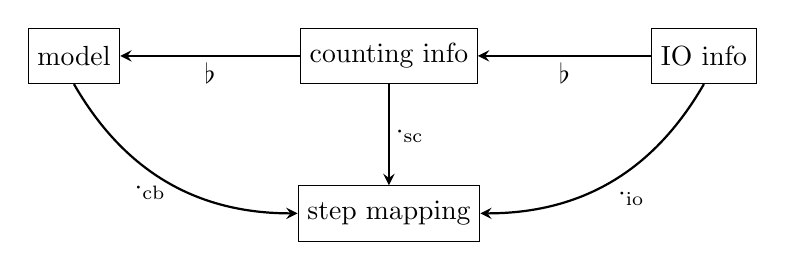
\begin{tikzpicture}[scale=2,>=stealth]
 \begin{scope}[every node/.style={rectangle,draw},minimum height=2em]
  \node (sm) at (+0,+0) { step mapping };
  \node (cb) at (-2,+1) { model };
  \node (sc) at (+0,+1) { counting info };
  \node (io) at (+2,+1) { IO info };
 \end{scope}
 \begin{scope}[every node/.style={inner sep=0.5ex}]
  \draw[thick] (cb.south) edge[->,bend right=30] node [auto,swap,inner sep=0] {$\stepmap\cdot_\mathrm{cb}$} (sm.west);
  \draw[thick] (sc.south) edge[->] node [auto] {$\stepmap\cdot_\mathrm{sc}$} (sm.north);
  \draw[thick] (io.south) edge[->,bend left=30] node [auto] {$\stepmap\cdot_\mathrm{io}$} (sm.east);
  \draw[thick] (sc.west) edge[->] node [auto] {$\flat$} (cb.east);
  \draw[thick] (io.west) edge[->] node [auto] {$\flat$} (sc.east);
 \end{scope}
\end{tikzpicture}\end{center}

In the definition of both $\varkappa=(q,\lambda,\pi)$ and $\mu=(q,\pi_1,K,H)$,
the only part that depends on $\omega$ is the probability model $q$. All other
parts are fixed as soon as the language model is instantiated, and are
therefore not subject to training. For many language models, it is sufficient
to choose $\Omega := \um_C(A|B)$ and $q = \operatorname{id}$ (i.~e.,~$q_\omega =
\omega$ for all $\omega$).  Applying Lemma~\ref{lemma:empirical2}, we see that
the empirical probability distribution for the complete-data corpus is an
element of $\stepmap\mu_\mathrm{io}(\omega)$ (and similar for the simple
counting step mapping). Since the EM algorithm only needs one element from
$\stepmap\mu_\mathrm{io}(\omega)$, we can use
\[
 \stepmap\mu'_\mathrm{io}(\omega) := \mbig\brc{ \widetilde{c\mnorm\dangle{\omega,\mu}} }
\]
instead, which is much less expensive to compute than the full $\argmax$.
